% Modified from AAAS Science LATEX template
% Use only LaTeX2e, calling the article.cls class and 12-point type.

\documentclass[11pt, a4paper, oneside]{article}
\usepackage{helvet}
\renewcommand{\familydefault}{\sfdefault}

\usepackage{graphicx}

\usepackage{caption}
\captionsetup{font=small}

\usepackage{scicite}

% Page setup

\topmargin 0.0cm
\oddsidemargin 0.2cm
\textwidth 16cm
\textheight 21cm
\footskip 1.0cm

\usepackage[legalpaper, portrait, margin=0.5in]{geometry}
% Abstract environment

\newenvironment{sciabstract}{%
\begin{quote} \bf}
{\end{quote}}

% Paper title

\title{
XPRESSyourself: Automating and Democratizing High-Throughput Sequencing
}


% Author info

\author
{
Jordan A. Berg,$^{1}$ Jonathan R. Belyeu,$^{2}$ Alex J. Bott,$^{1}$ Jeffrey T. Morgan,$^{1}$ Yeyun Ouyang,$^{1}$\\
Jason Gertz,$^{3}$ Michael T. Howard,$^{2}$ Aaron R. Quinlan,$^{2,4,5}$ Jared P. Rutter$^{1,6\ast}$\\
\\
\normalsize{$^{1}$Department of Biochemistry, University of Utah, Salt Lake City, UT, USA, 84112}\\
\normalsize{$^{2}$Department of Human Genetics, University of Utah, Salt Lake City, UT, USA, 84112}\\
\normalsize{$^{3}$Department of Oncological Sciences, University of Utah, Salt Lake City, UT, USA, 84112}\\
\normalsize{$^{4}$USTAR Center for Genetic Discovery, University of Utah, Salt Lake City, UT, USA, 84112}\\
\normalsize{$^{5}$Department of Biomedical Informatics, University of Utah, Salt Lake City, UT, USA, 84112}\\
\normalsize{$^{6}$Howard Hughes Medical Institute, University of Utah, Salt Lake City, UT, USA, 84112}\\
\\
\normalsize{$^\ast$To whom correspondence should be addressed; E-mail: rutter@biochem.utah.edu.}
}

% Include the date command, but leave its argument blank.

\date{}



%%%%%%%%%%%%%%%%% END OF PREAMBLE %%%%%%%%%%%%%%%%


% Initialize use of code blocks with syntax highlighting

\usepackage{listings}
\usepackage{color}

\definecolor{codegreen}{rgb}{0,0.6,0}
\definecolor{codegray}{rgb}{0.5,0.5,0.5}
\definecolor{codepurple}{rgb}{0.58,0,0.82}
\definecolor{backcolour}{rgb}{0.95,0.95,0.92}

\lstdefinestyle{mystyle}{
    backgroundcolor=\color{backcolour},
    commentstyle=\color{codegreen},
    keywordstyle=\color{magenta},
    numberstyle=\tiny\color{codegray},
    stringstyle=\color{codepurple},
    basicstyle=\footnotesize,
    breakatwhitespace=false,
    breaklines=true,
    captionpos=b,
    keepspaces=true,
    numbers=left,
    numbersep=5pt,
    showspaces=false,
    showstringspaces=false,
    showtabs=false,
    tabsize=2
}

\lstset{style=mystyle}

\begin{document}

% Double-space the manuscript.
\baselineskip24pt

% Make the title.
\maketitle



% Place your abstract within the special {sciabstract} environment.

\begin{sciabstract}
  With the advent of high-throughput sequencing platforms, expression profiling is becoming common-place in medical research. However, for the general user, often someone who ends up outsourcing their bioinformatics, a computational overhead exists. The XPRESSyourself suite aims to remove these barriers and create a tools to help standardize and increase throughput of data processing and analysis. The XPRESSyourself suite is currently broken down into two software packages. The first, XPRESSpipe, automates the pre-processing, alignment, quantification, normalization, and quality control of single-end and paired-end RNAseq, as well as ribosome profiling sequence data. The second, XPRESStools, is a Python toolkit for expression data analysis, compatible with private or public microarray and RNAseq datasets. This software suite is designed where features can easily be modified, and additional packages can be included for processing of other data types in the future, such as CHIPseq or genome alignment. Currently, this package offers several new tools for ribosome profiling and general RNA-seq.
  \newline\\
  \normalfont XPRESSyourself is freely available on GitHub: https://github.com/XPRESSyourself\\
\end{sciabstract}


\section{Introduction}

High-throughput profiling of gene expression data has revolutionized biomedical, industrial and basic science research. Within the last two decades, RNA-seq as found itself the forerunner technology for highest quality expression profiling, as it can measure relative transcript abundance, differential splice variants, sequence polymorphisms, and more. This technology has also been adopted to create technologies such as single-cell RNA-seq, capable of assaying the transcriptional profile cell by cell; and ribosome profiling, which measures ribosome occupancy and translation efficiency.

While vast strides have been made to these technologies, various bottlenecks still exist. For example, while more and more researchers are becoming accustomed to these technologies, learning the bioinformatics portion of sequencing possesses its own learning curve and often efficiency is lacking in how sequencing reads are processed and analyzed. Also for these users, they may not be aware of which tools are accepted as the standard in the field or which analyses they should be perform. They may also lack the experience to process their sequencing libraries rapidly or may not know all the in-between steps that are not always explicitely stated in protocols.

While several pipelines have emerged over the last several years that have been built to tackle various aspects of these bottlenecks, most are not widely used or usable by the average wet-bench researcher. Some are difficult to install or use, often they break easily or do not perform well. Rarely do these tools offer anything new to help overcome emerging challenges in the field.

In response to these issues surrounding the automation and democratization of sequencing technology, we created the XPRESSyourself bioinformatics suite for processing and analyzing high-throughput expression data. In creating this tool, we focused on five aspects in order to create an easy, reliable tool where large barriers-to-entry would be elimiated. These were create a tool that was useful, usable, reliable, efficient, and flexible.

\begin{enumerate}
  \item We wanted the software we created to be useful for a broad audience, where the bulk of processing and analysis desired by a general user would be covered. We wanted to use pre-existing tools that were fast and accurate. We also wanted to provide additional, new tools that would be of use to the general RNA-seq community, which will be discussed in more detail later.

  \item We wanted to create a software package that was easy to use. To do so, we made the tools installable by a single command in the command line interface (CLI) using the Conda and PyPi package managers. We also included thorough external documentation hosted on readthedocs that outlines use and considerations for each tool, as well as provides several examples of how to use each tool. Internally in the CLI-packages, summary documentation has been included by way of the help interface. Jupyter notebooks are also created and installed with the software that provide example analyses that can be easily modified and run.

  \item To create a reliable pipeline and analysis package, we use the most current state-of-the-art software tools that have undergone robust benchmarking. We utilize a two-pass RNA-seq alignment process to provide the best coverage around splice sites. We also built the RNA-seq pipeline according to The Cancer Genome Atlas (TCGA) standards. While this technology will no doubt improve over the years, the software is structures in a way for easy modification for addition of tools or substitution of software.

  \item In order to make the most efficient package possible, by default XPRESSyourself optimizes use of computing cores to ensure all available are utilized when possible. Additionally, for analysis tools processing large files, we utilize a data matrix chunking method, where a dataset is portioned off into a number equal to the number of cores available, and processes each parallely before rejoining the data chunks.

  \item Flexibility is paramount in creating a tool that can be widely used and built upon. The general structure of the software was designed to make it easy to add or remove features. We envision as this suite of tools is more widely adopted by the RNAseq community, modules will be added to handle other sequencing platforms, such as genome sequencing, CHIPseq, and so on.
\end{enumerate}

With XPRESSyourself, the user is provided with a complete suite of software to handle pre-processing, aligning, and quantifying reads, performing quality control via various meta-analyses of pre- and post-processed reads, and tools to perform the bulk of sequence analysis with enough flexibility to generate professional, figure-worthy images.

\section{Materials and Methods}

\subsection{XPRESSpipe}
XPRESSpipe pipelines for single-end RNA-seq, paired-end RNA-seq, and ribosome profiling offer a handful of tunable parameters to the user, while keeping most hidden to maintain TCGA alignment standards. In the future it is feasible that additional tunable parameters will be added. Table \ref{Tab:xpresspipe} outlines these parameters.

\captionof{table}{Summary of XPRESSpipe pipeline arguments.\label{Tab:xpresspipe}}
\begin{tabular}{p{5cm}p{13cm}}
 \textbf{Arguments} & \textbf{Description} \\
 \hline
 \textbf{Required} & \\
 \hline
 -i, --input & Path to input directory \\
 \hline
 -o, --output & Path to output directory \\
 \hline
 -r, --reference & Path to parent organism reference directory \\
 \hline
 -t, --reference\_type & GTF, refFlat, etc. type (i.e. ``DEFAULT", ``CODING", ``CODING\_TRUNCATED") \\
 \hline
 -e, --experiment & Experiment name \\
 \hline
 \textbf{Optional} & \\
 \hline
 -a, --adaptors & Specify adaptor as string (only one allowed) -- if ``None" is provided, software will attempt to auto-detect adaptors -- if ``POLYX" is provided as a single string in the list, polyX adaptors will be trimmed \\
 \hline
 -q, --quality & PHRED read quality threshold (default: 28) \\
 \hline
 --min\_length & Minimum read length threshold to keep for reads (default: 18) \\
 \hline
 --output\_bed & Include option to output BED files for each aligned file \\
 \hline
 --output\_bigwig & Include flag to output bigwig files for each aligned file \\
 \hline
 --method & Normalization method to perform (options: ``RPM", ``RPKM", ``FPKM", ``LOG") \\
 \hline
 --batch & Include path and filename of dataframe with batch normalization parameters \\
 \hline
 --sjdbOverhang & Sequencing platform read-length for constructing splice-aware reference previously (see documentation for more information) \\
 \hline
 --downstream & Number of nucleotides to track after the landmark (default: 200) \\
 \hline
 -m, --max\_processors & Number of max processors to use for tasks (default: No limit) \\
\end{tabular}
\newline

\subsubsection{Installation}
General installation of XPRESSpipe is handled by the package manager, Anaconda{}, which is easy to download and install (https://www.anaconda.com/distribution/). XPRESSpipe can be installed using the following command:
\newline

% Install XPRESSpipe code block
\begin{lstlisting}[language=bash, caption=curateReference example]
$ conda install -c bioconda XPRESSpipe
\end{lstlisting}

% Software dependencies table
\captionof{table}{Summary of dependency software, accession location, and purpose in the XPRESSpipe package.\label{Tab:packages}}
\begin{tabular}{p{2.4cm}p{7.5cm}p{6.5cm}}
 \textbf{Package} & \textbf{URL} & \textbf{Purpose} \\
 \hline
 fastp & https://github.com/OpenGene/fastp & Read pre-processing \\
 \hline
 ucsc-gtftogenepred & http://hgdownload.cse.ucsc.edu/admin/exe/ & Create refFlat reference file used in meta-analysis \\
 \hline
 STAR & https://github.com/alexdobin/STAR & Reference curation and read alignment \\
 \hline
 samtools & http://www.htslib.org/ & Alignment file manipulation \\
 \hline
 bedtools & https://github.com/arq5x/bedtools2 & Alignment file manipulation \\
 \hline
 deeptools & https://github.com/deeptools/deepTools & Alignment file manipulation \\
 \hline
 htseq & https://github.com/simon-anders/htseq & Read quantification \\
 \hline
 fastqc & https://www.bioinformatics.babraham.ac.uk/ projects/fastqc/ & Quality Control \\
 \hline
 multiqc & https://multiqc.info/ & Quality Control \\
 \hline
 picard & https://broadinstitute.github.io/picard/ & Transcript meta-analysis \\
 \hline
 plastid & https://github.com/joshuagryphon/plastid & Periodicity meta-analysis \\
\end{tabular}
\newline

XPRESSpipe is built upon several pre-established software packages, listed in Table \ref{Tab:packages}. These packages will be automatically installing using the Anaconda package manager; however, if installing manually, these packages will need to be installed by the user.

\subsubsection{Inputs}
While inputs will vary sub-module to sub-module, and further information can be found in the documentation (https://xpresspipe.readthedocs.io/en/latest/) or by entering ``xpresspipe \textless sub-module name\textgreater \ --help", a few points of guidance are important to consider.

\begin{itemize}
\item Single-end reads should end in ``.fa", ``.fasta", ``.txt"
\item Paired-end reads should end in ``.read1/2.suffix" or ``.r1/2.suffix"
\item The transcriptome reference file should be a valid GTF file and should be named ``transcripts.gtf"
\item If specifying a group of fasta files to use for alignment or reference curation, the directory containing this files cannot contain any other files ending in ``.txt" or ``.fa"
\end{itemize}

\subsubsection{Reference Curation}
One of the first preparatory steps of RNAseq alignment is curating a reference transcriptome for the aligner to map reads to. For the purposes of XPRESSpipe, a STAR reference should be created. However, for the purposes of several meta-analyses and more specific mapping, a STAR{} reference alone is not enough. For example, if one is aligning ribosome profiling reads and wishes to avoid mapping reads to the first 45 nucleotides in order to not quantify the inherent 5' biases in library preparation{}, a truncated transcriptome reference needs to be used when counting reads to transcripts. Additionally, if one wishes to only quantify reads to the coding portions of the transcriptome, a custom reference file needs to be created. While each of these steps are available as stand-alone sub-modules, all potential reference files, including STAR files, modified transcriptome files, and other meta-analysis files can be created by running the ``curateReference" command. An example is shown below for creating a ribosome profiling-ready reference XPRESSpipe directory. The following assumes one is avoiding mapping to the first 45 nucleotides, will only quantify to protein coding regions, and is tailored for mapping 50-bp single-end RNA-seq reads. As this can be a time-consuming process, we will leave the ``--max\_processors" argument as default in order to utilize all cores available to the computing unit.
\newline
\begin{lstlisting}[language=bash, caption=curateReference example]
$ xpresspipe curateReference -o /path/to/output/location/
                              -f /path/to/fasta/genome/files/
                              -g /path/transcripts.gtf
                              --truncate_amount 45
                              --sjdbOverhang 49
\end{lstlisting}

While current available arguments are limited, the design is simple enough where arguments could be added easily to give more control over STAR reference creation; however, current setting align with TCGA standards.

\subsubsection{Read Processing}
While all intermediate steps of the pipelines can be run singly, we will describe the outline of the software in the context of the pipelines.

\begin{enumerate}
  \item Trim: The first step in read processing is removing reads of artifacts for the library preparation process. These are most often adaptor sequences that were ligated to each read during the preparatory steps, which will not have homology to the organism's reference sequence. As sequencers are only so accurate, another common artifact are base calls that are statistically not confident. Therefore, in the first step of read processing, it is important to remove these sequences from each read to allow for proper alignment of reads to the reference. XPRESSpipe begins by trimming reads of adaptors, low quality bases, and reads that are too short using fastp, a more recent, faster trimming package that has improved alignable read output{}. Adaptor sequence, base quality, and read length are all adjustable parameters available to the user. Descriptions of the options can be found in Table \ref{Tab:xpresspipe}.
  \item Align: After sequencing reads have been trimmed of artifacts, the next step is to determine what transcripts these reads originated from to quantitate expression levels. This is done through alignment of each read to the reference transcriptome. XPRESSpipe uses STAR{} for this process as it has consistently proven itself as a fast and accurate alignment tool{}, such that it has been chosen as the TCGA standard alignment software. Alignment is made easy by generating a reference directory using XPRESSpipe's ``curateReference" sub-module. XPRESSpipe then performs a two-pass alignment to maximize alignment to splice junctions. In the first pass, STAR identified potential splice junctions for each sample, generates a reference taking these sites into account, then uses this reference to remap reads to the reference. Afterwards, some file processing is performed to generate the appropriate output files and formats for downstream steps.
  \item Count: Once reads have been aligned and genome coordinates have been determined, these reads need to be quantified. XPRESSpipe uses htseq{} for this purpose. In this step, reads coordinates along the genome are mapped to the reference transcriptome. If a coding-only or truncated reference was created during the reference curation, this will be used for the quantification of transcipts. By default, htseq behavior conforms to TCGA standards by being strand agnostic, mapping assuming reads were sorted by name, and by using the intersection-nonempty method for handling reads overlapping multiple genes.
  \item Normalization: As RNA-seq measurements are only relative, they are subject to sample and batch effects. These can arise from different people preparing libraries, one person preparing libraries on different days, or are just inherent in differences in total reads per sample a given chip sequences. In order to remove sample effects arising per sequence chip, it is important to perform normalization. Reads-per-million (RPM) normalization controls for these sample effects. Reads-per-kilobase-million (RPKM) or Fragments-per-kilobase-million (FPKM) performs the same RPM normalization, but additionally normalizes for transcript length as longer transcripts will appear to have more reads aligning to these transcripts normally. Batch effect normalization controls for library to library variances. These normalization options are available in the XPRESSpipe arguments for each pipeline (see Table \ref{Tab:xpresspipe}).
  \item Quality Control: It is important to perform quality control of sequencing sample to ensure they are reliable and their biological insight can be trusted. XPRESSpipe performs a variety of quality control measures. fastqc{} runs a gambit of quality control measures and multiqc summarizes these and metrics from trimming, aligning, and so on. The ``readDistribution" sub-module will take the read size distributions for each library, as this can be informative, especially in the case of ribosome profiling, to ensure the proper read length was enriched in the sequencing library. The ``metagene" sub-module will summarize read distribution along a representative transcript to highlight any sequencing biases, such as an enrichment of reads on the 3' end indicative of poor library preparation. The ``periodicity" sub-module will take the most enriched read length from ribosome profiling footprint libraries and map the P-site of the ribosome to investigate the 3 nucleotide phasing characteristic of the translating ribosome. Each of these sub-modular quality functions will summarize their results in a single PDF for quick reference by the user.
  \item Analyses:
        prober

        diffex

\end{enumerate}

pipeline
  run singly or all together
  normalization / batch effect

\subsubsection{Outputs}
output
  minimal but enough to get clear picture
  optional outputs

  \begin{figure}
    \fbox{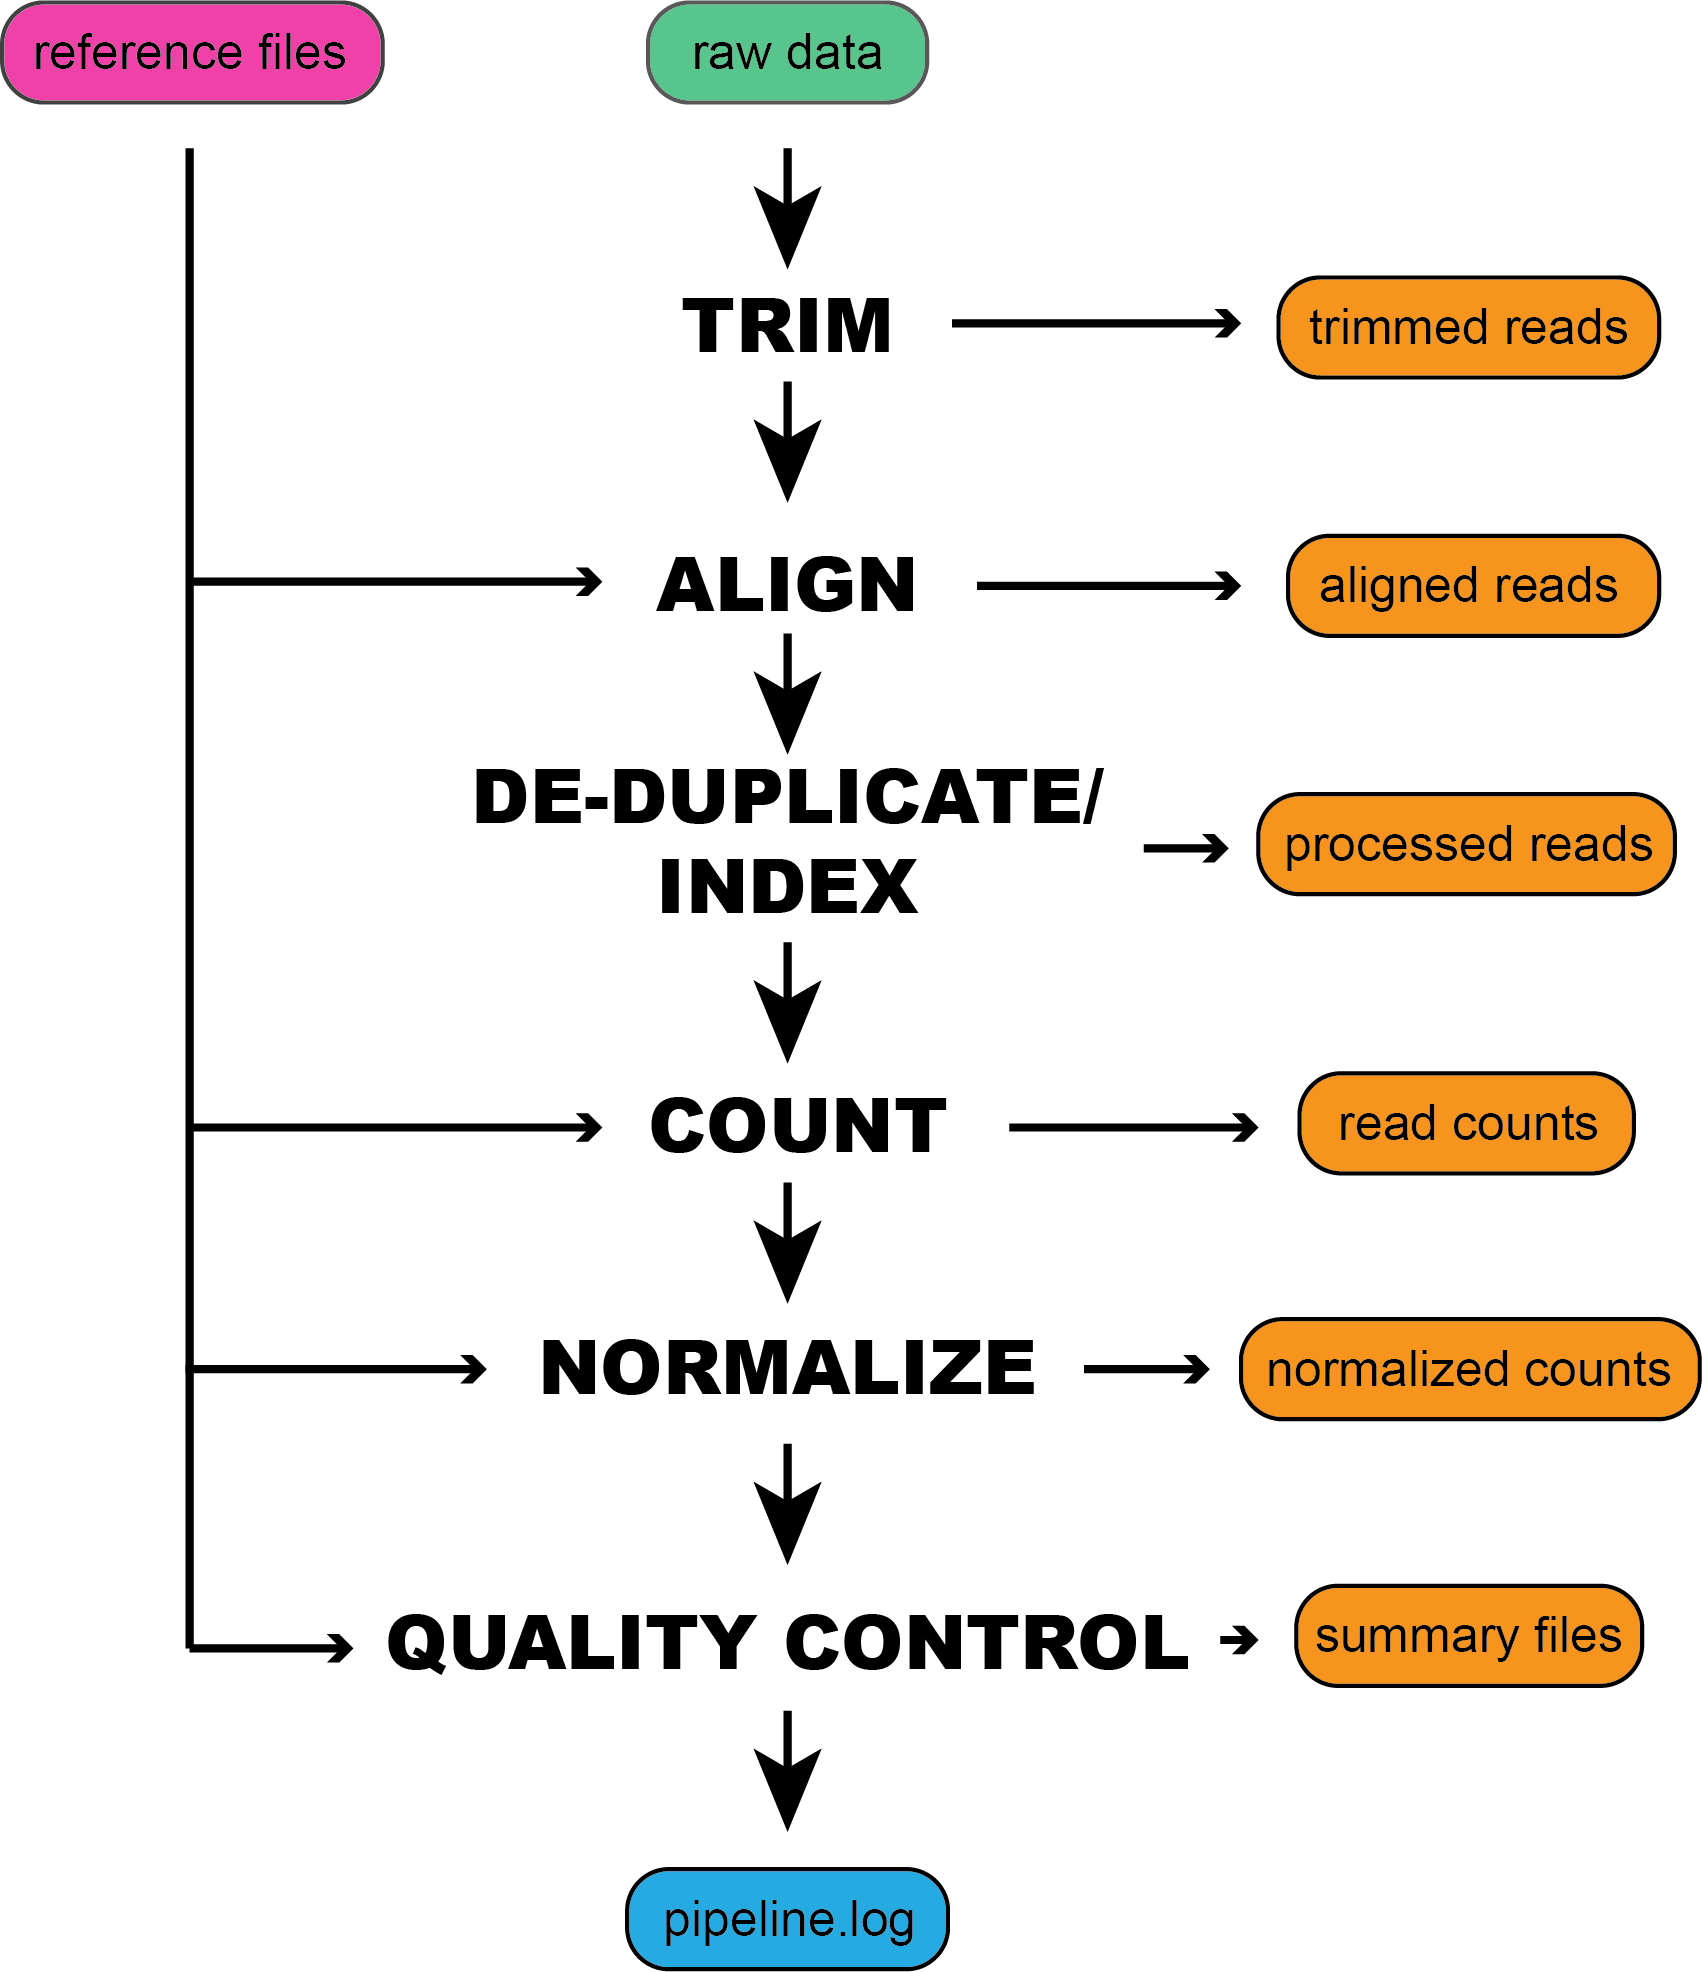
\includegraphics[width=\linewidth]{figures/xpresspipe_overview.png}}
    \caption{A schematic of XPRESSpipe outputs. Input, output, and often reference directories are specified and each stage of processing or analysis is given a separate directory.}
    \label{fig:outputs}
  \end{figure}

Figure \ref{fig:outputs} provides an example of output file scheme for XPRESSpipe.


\subsubsection{Quality Control}
quality control
  read distribution
  meta-gene
  periodicity

\subsubsection{Analyses}
prober
Deseq

\subsection{XPRESStools}

\subsubsection{Getting Data}

\subsubsection{Normalizing and Formatting Data}

\subsubsection{Analyzing Data}

\subsection{Unit Testing and Code Coverage}
New tools will require new tests to maintain code Coverage

\subsection{Availability}
Open source community
GitHub
Version Control
Singularity


\section*{Results and Discussion}

\subsection{Benchmarking}

\subsection{Example Data Walkthrough}

\subsection{Cost Analysis}

\subsection{Summary}


\bibliography{scibib}

\bibliographystyle{Science}


\section*{Acknowledgments}
J.A.B. received support from the National Institute of Diabetes and Digestive and Kidney Diseases (NIDDK) Inter-disciplinary Training Grant T32 Program in Computational Approaches to Diabetes and Metabolism Research, 1T32DK11096601 to Wendy W. Chapman and Simon J. Fisher.


\section*{Contributions}
\begin{tabular}{ l l }
 Conceptualization & J.A.B. \\
 \hline
 Supervision & M.T.H., J.G., A.R.Q., J.P.R. \\
 \hline
 Project Administration & J.A.B. \\
 \hline
 Investigation & J.A.B. \\
 \hline
 Formal Analysis & J.A.B. \\
 \hline
 Software & J.A.B. \\
 \hline
 Methodology & J.A.B. \\
 \hline
 Validation & J.A.B., A.J.B. Y.O. \\
 \hline
 Data Curation & J.A.B. \\
 \hline
 Resources & J.A.B., J.P.R. \\
 \hline
 Funding Acquisition & J.A.B., J.P.R. \\
 \hline
 Writing - Original Draft & J.A.B. \\
 \hline
 Writing - Review \& Editing & J.A.B., M.T.H., J.G., A.R.Q., J.P.R. \\
 \hline
 Visualization & J.A.B.
\end{tabular}

\end{document}
